\documentclass[11pt,a4paper]{article}
\usepackage[utf8]{inputenc}
\usepackage[T1]{fontenc}
\usepackage[english]{babel}
\usepackage{fancyhdr}
\usepackage{kpfonts}
\usepackage[margin=.8in]{geometry}
\usepackage{exsheets}
\usepackage{amsmath, amssymb, amsfonts}
\usepackage{enumerate}
\usepackage{tikz}
\usetikzlibrary{arrows, decorations.text}

\pagestyle{fancy}
\renewcommand{\headrulewidth}{2pt}
\fancyhead[L]{Epita - BING}
\fancyhead[R]{2016}

\fancyfoot[C]{\textbf{\thepage}} 
\fancyfoot[L]{}

\SetupExSheets{subtitle-format = \Large\scshape}
\SetupExSheets{headings-format = \large\bfseries}
\SetupExSheets{headings = block-subtitle}
\SetupExSheets{solution/print=true}
\SetupExSheets{question/type=exam}
\RenewQuSolPair{question}[name={\large Exercise}]{solution}

\begin{document}
\begin{center}
  {\Large \textbf{Networks and Flows on Graphs}}\\
  \vspace{10pt}
  {\Large \textit{Exercise Sheet}}
\end{center}
\rule{\textwidth}{2pt}
\vspace{\baselineskip}

\section{Basics on Graphs}

\begin{question}[subtitle={Adjacency and Incidence Matrices}]
  Let $M$ be the matrix
  \[
  M = \begin{pmatrix}
    0 & 1 & 0 & 1 & 0 \\
    0 & 0 & 1 & 0 & 0 \\
    0 & 0 & 0 & 0 & 1 \\
    0 & 0 & 1 & 0 & 1 \\
    0 & 0 & 0 & 0 & 0
  \end{pmatrix}
  \]
  representing a graph $G$ having vertices $A$, $B$, $C$, $D$, $E$. 
  \begin{enumerate}
  \item Draw the graph having adacency matrix $M$.
  \item What is the incidency matrix of $G$?
  \item Compute $M^2$, $M^3$ and $M^4$. Can you tell what non-zero
    coefficients correspond to?
  \item Knowing that $M^{[k]}$ is the $k$-th boolean power of $M$,
    compute $M^{[2]}$, $M^{[3]}$ and $M^{[4]}$. Can you give a meaning
    to these matrices?
  \item Compute
    $A = I \oplus M \oplus M^{[2]} \oplus M^{[3]} \oplus M^{[4]}$,
    where $\oplus$ is the boolean sum. What does $A$ stand for?
  \end{enumerate}
\end{question}

\begin{question}[subtitle={Degrees and Cycles}]
  Consider the following graph, subsequently named $G$:
  \begin{center}
    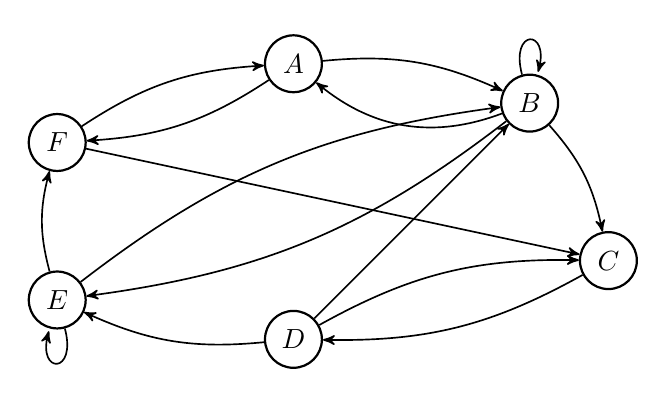
\begin{tikzpicture}
        [minimum width={width("b")+1.5em},
        vertex/.style={circle, draw=black, fill=white, thick},
        arr/.style={->,>=stealth',semithick}]
        \node (C) at (7, 3.5) [vertex] {$C$};        
        \node (A) at (3, 6) [vertex] {$A$};
        \node (F) at (0, 5) [vertex] {$F$}
           edge[arr, bend left=15] (A)
           edge[arr] (C);
        \node (E) at (0, 3) [vertex] {$E$}
           edge[arr, bend left=15] (F)
           edge[loop below, semithick, >=stealth'] (E);
        \node (B) at (6, 5.5) [vertex] {$B$}
           edge[arr, bend left] (A)
           edge[loop above, semithick, >=stealth'] (B)
           edge[arr, bend left=15] (C)
           edge[arr, bend left=15] (E);
        \node (D) at (3, 2.5) [vertex] {$D$}
           edge[arr] (B)
           edge[arr, bend left=15] (C)
           edge[arr, bend left=15] (E);
        \path (C) edge[arr, bend left=15] (D);
        \path (A) edge[arr, bend left=15] (F);
        \path (A) edge[arr, bend left=15] (B);
        \path (E) edge[arr, bend left=15] (B);
     \end{tikzpicture}
  \end{center}
  \begin{enumerate}
  \item Compute inner and outer degrees of each one of the vertices.
  \item Give an example of a simple path which is not elementary.
  \item Is there a hamiltonian circuit in $G$?
  \item Draw the oriented graph corresponding to $G$.
  \item Is $G$ connected? strongly connected?
\end{enumerate}
\end{question}

\begin{question}[subtitle={Railways}]
  Consider the following railway track :
  \begin{center}
    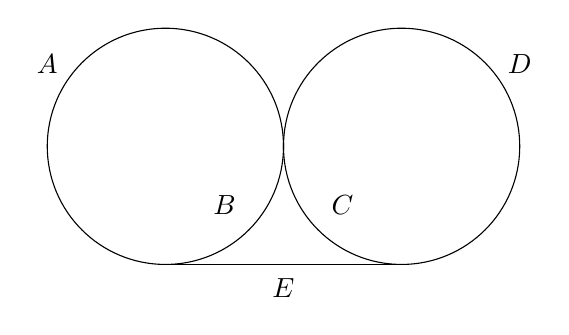
\begin{tikzpicture}[scale=1.5]
      \draw (0,0) circle (1cm);
      \draw (2,0) circle (1cm);
      \draw (0, -1) -- (2, -1);
      \node at (1, -1.2) {$E$};
      \node at (.5, -.5) {$B$};
      \node at (1.5, -.5) {$C$};
      \node at (3, .7) {$D$};
      \node at (-1, .7) {$A$};
    \end{tikzpicture}
  \end{center}
  Each cross-point on the railway track has two available
  positions. Could you explain why trains will eventually never go
  through section $E$? What would happen if we added a section $F$
  symmetric to $E$?
\end{question}

\begin{question}[subtitle={Strongly Connected Components}]
  Give the strongly connected components of the following graph :
    \begin{center}
    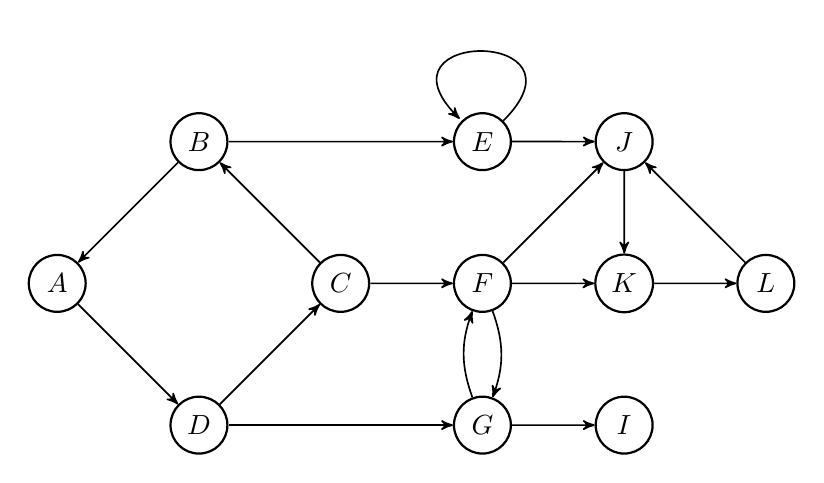
\begin{tikzpicture}
        [minimum width={width("b")+1.5em},
        vertex/.style={circle, draw=black, fill=white, thick},
        arr/.style={->,>=stealth',semithick}, scale=1.8]
        \node (I) at (4, 1) [vertex] {$I$};  
        \node (L) at (5, 2) [vertex] {$L$};              
        \node (K) at (4, 2) [vertex] {$K$}
          edge[arr] (L);        
       \node (J) at (4, 3) [vertex] {$J$}
          edge[arr] (K);        
        \node (G) at (3, 1) [vertex] {$G$}
          edge[arr] (I);
        \node (F) at (3, 2) [vertex] {$F$}
          edge[arr, bend left=20] (G)
          edge[arr] (K)
          edge[arr] (J);
        \node (E) at (3, 3) [vertex] {$E$}
          edge[arr] (J)
          edge[loop, semithick, >=stealth'] (E);                
        \node (A) at (0, 2) [vertex] {$A$};
        \node (B) at (1, 3) [vertex] {$B$}
          edge[arr] (A)
          edge[arr] (E);
        \node (C) at (2, 2) [vertex] {$C$}
          edge[arr] (B)
          edge[arr] (F);        
        \node (D) at (1, 1) [vertex] {$D$}
          edge[arr] (C)
          edge[arr] (G);
        \path (A) edge[arr] (D);
        \path (G) edge[arr, bend left=20] (F);
        \path (L) edge[arr] (J);
     \end{tikzpicture}
  \end{center}
\end{question}

\section{Network Flows}

\begin{question}[subtitle={Flows}]
  Ports $C$, $D$ and $E$ are respectively in need of $9$, $12$ and $7$
  containers of a given good $X$. They are connected to ports $A$ and
  $B$, which have each $10$ containers of $X$ that are ready to
  go. There are currently $4$ shipping routes : 
  \begin{itemize}
  \item from $A$ to $C$ and $A$ to $D$ having respective maximal
    shipping capacities of $7$ and $4$ containers ;
  \item from $B$ to $C$ and $B$ to $E$ having respective maximal
    capacities of $5$ and $5$.
  \end{itemize}
  \begin{enumerate}
  \item Is it possible to satisfy all demands?
  \item How can one organise the traffic in order to ensure a maximum
    total number of containers? You're expected to start with initial
    solution sending $7$ containers through route $AC$. You are to
    update initial solution using Ford-Fulkerson algorithm. What is
    the mimimum cut corresponding to max flow solution?
  \end{enumerate}
\end{question}

\begin{question}[subtitle={Pairings}]
  During a bal, $5$ men and $5$ women are looking forward to
  dance. We're given the hard task of mathcing up the highest number
  of couples (gender assymetric ones) taking the below compatibility
  table
    \begin{center}
    \renewcommand{\arraystretch}{1.5}
    \begin{tabular}{r|c|c|c|c|c}
      & Marie & Claire & Suzanne & Anne & Jeanne \\
      \hline
      Joseph &  $\spadesuit$ &  $\heartsuit$ & $\spadesuit$ & $\spadesuit$ & $\spadesuit$ \\
      \hline
      Paul &  $\heartsuit$ & $\spadesuit$ & $\spadesuit$ & $\spadesuit$ & $\spadesuit$  \\
      \hline
      Luc &  $\heartsuit$ & $\heartsuit$  & $\spadesuit$ & $\spadesuit$ & $\spadesuit$  \\
      \hline
      Bernard & $\heartsuit$ & $\heartsuit$  &  $\spadesuit$ & $\spadesuit$ & $\heartsuit$  \\
      \hline
      Francois & $\spadesuit$  & $\spadesuit$  & $\heartsuit$ & $\heartsuit$ & $\heartsuit$ \\
    \end{tabular}
  \end{center}
  \begin{enumerate}
  \item What is the graph best representing this matching problem?
  \item How can network flows formalism help you solve this matching problem?
  \end{enumerate}
\end{question}


\section{Optimal Transportation Programs}

\begin{question}[subtitle={Transportation Program}]
  A road transport company has to ship a number of goods out of three
  docks $O_1$, $O_2$ and $O_3$ to $4$ destinations $D_1$, $D_2$, $D_3$
  and $D_4$. Each dock has $10$ available shipments and the needed
  shipments at each destination are $7$, $4$, $14$ and $5$
  respectively at $D_1$, $D_2$, $D_3$ and $D_4$. The following table
  sums up the costs of each route between a given dock and any
  destination
  \begin{center}
    \renewcommand{\arraystretch}{1.5}
    \begin{tabular}{c|c|c|c|c}
      & $D_1$ & $D_2$ & $D_3$ & $D_4$ \\
      \hline
      $O_1$ & 5 & 10 & 11 & 21 \\
      \hline
      $O_2$ & 6 & 8 & 11 & 2 \\
      \hline
      $O_3$ & 21 & 12 & 3 & 5 \\
    \end{tabular}
  \end{center}
  The company is looking for the least cost transportation program.
  \begin{enumerate}
  \item Give a basic solution to this transportation problem using the
    Balas-Hammer heuristic. What is the cost of this solution?
  \item What is the optimal transportation program? Is the optimum unique?
  \item Following improvements on the connection between $O_2$ and
    $D_1$, cost to go from $O_2$ to $D_1$ has gone down from $4$ to
    $6$. Is the previous solution still optimal? If not find the new
    optimal solution.
  \end{enumerate}
\end{question}

\section{Paths Optimisation}

\begin{question}[subtitle={Along GR $58$}]
  At Cervières one can find the map below, it sums the level of
  difficulty going through any of the pictured paths. You goal is to
  plan the hike to the Queyras where a \emph{fondue} is waiting and a
  bottle of \emph{VEP}.
  
  The total difficulty of a given hike is the sum of difficulties of
  each elememtary route. 
  \begin{enumerate}
  \item Using the Ford algorithm compute the easiest hike from
    Cervières to any other stop. What is the easiest hike from
    Cervières to Queyras?
  \item Is the Ford algorithm the best choice one can make to solve
    the previous issue, of going from Cervières to Queyras on the
    easiest hike. How would you do otherwise?
  \item If your aim was to break the record of the toughest hike, what
    route would you take?
  \end{enumerate}
  
\end{question}

\begin{question}[subtitle={Shortest Path Problem}]
  Using the Floyd-Warshall algorithm give the longest paths in between
  any two vertices of the following grahps
    \begin{center}
    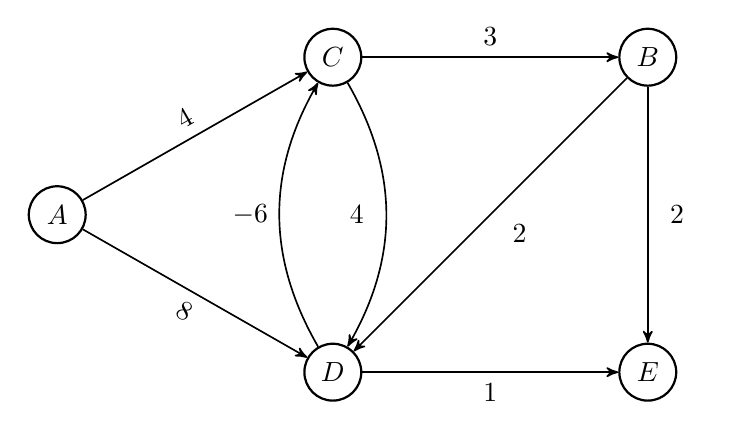
\begin{tikzpicture}
        [minimum width={width("b")+1.5em},
        vertex/.style={circle, draw=black, fill=white, thick},
        arr/.style={->,>=stealth',semithick}]
        \node (E) at (13,3) [vertex] {$E$};
        \node (D) at (9,3) [vertex] {$D$}
           edge[
           arr, 
           postaction={
             decorate, 
             decoration={raise=-2.5ex, text along path, text align=center, text={1}}
           }
           ] 
           node[below] {} (E);
        \node (B) at (13,7) [vertex] {$B$}
           edge[arr] node[right] {$2$} (E)
           edge[arr]  node[below right] {$2$} (D);
        \node (C) at (9,7) [vertex] {$C$}
           edge[
           arr, 
           postaction={
             decorate, 
             decoration={raise=1ex, text along path, text align=center, text={3}}
           }
           ] 
           node[above] {} (B)
           edge[arr, bend left] node[left] {$4$} (D);
        \node (A) at (5.5,5) [vertex] {$A$}
           edge[           
           arr, 
           postaction={
             decorate, 
             decoration={raise=1ex, text along path, text align=center, text={4}}
           }
           ] 
           node[above] {} (C)
           edge[
           arr, 
           postaction={
             decorate, 
             decoration={raise=-2.5ex, text along path, text align=center, text={8}}
           }
           ] 
           node[below] {} (D);
           \path (D) edge[arr, bend left] node [left] {$-6$} (C);
     \end{tikzpicture}
  \end{center}
  Does looking for shortest paths in between any two vertices of this
  graph make sense?
\end{question}

\section{Scheduling}

\begin{question}[subtitle={Project Scheduling}]
  A project is split into $8$ elementary tasks. In the table below, we
  sum up the needed time (in days) to accomplish a given task and the
  tasks one has to go through beforehand.
    \begin{center}
    \renewcommand{\arraystretch}{1.5}
    \begin{tabular}{|c|c|c|}
      \hline
      Tasks & Pre-tasks & Durations  \\
      \hline
      a & -- &  $2$ \\
      \hline
      b & --  & $3$ \\
      \hline
      c & --  & $7$ \\
      \hline
      d & b, h  & $4$ \\
      e & a  & $10$ \\
      \hline
      f & a, d  & $6$ \\
      \hline
      g & b, c  & $5$ \\
      \hline
      h & --  & $1$ \\
      \hline
    \end{tabular}
  \end{center}
  Our aim is to find a project scheduling that minimizes the total
  duration of the project.
  \begin{enumerate}
  \item Use the potential method to solve previous problem. Point out
    the earliest starting date for each task, the critical path and
    its duration. Draw the corresponding potential graph.
  \item Figure out the latest possible start of each task. 
  \item Give up a PERT graph modeling the previous scheduling problem
    without introducing any external constraints (you'll need a number
    of virtual tasks). Recover back previous cirtical paths using
    relevant algorithms.
  \end{enumerate}
  
\end{question}


\begin{question}[subtitle= {Assisting the Director}]
  A movie producer is looking forward to plan his next movie to
  be. Here are the list of tasks to be done for the movie to get out
  on the screens. 
  \begin{center}
    \renewcommand{\arraystretch}{1.5}
    \begin{tabular}{|c|l|c|p{5cm}|}
      \hline
      Task Code & Task detail & Duration & Precedency \\
      \hline
      A & Writing the scenario  & 30  &   \\
      \hline
      B & Casting  & 12  & Can only start 15 days after A starts  \\
      \hline
      C & Choosing shooting place  & 8  &  Can only start 20 days after A starts \\
      \hline
      D & Technical cut  & 4  & A and C have to be finished  \\
      \hline
      E & Preparing set  & 7  & C and D have to be finished  \\
      \hline
      F & Exterior shooting  & 10  & A, B, C and D have to be finished  \\
      \hline
      G & Interior shooting  & 12  & D, E and F have to be finished  \\
      \hline
      H & Synchronisation  & 3  & F and G have to be finished  \\
      \hline
      I & Editing  & 14  & H has to be finished  \\
      \hline
      J & Sound background  & 7  & Can only start 3 days after the start of I and after H is finished  \\
      \hline
      K & Mixing  & 6  & I and J have to be finished  \\
      \hline
      L & Answer print  & 1  & Can only start 2 days after end of K  \\
      \hline       
    \end{tabular}
  \end{center}
  \begin{enumerate}
  \item Using the MPM model, give the earliest dates at which each
    task can be done. What is the critical path?
  \item Delete superfluous precedency constraints obtained by transitivity.
  \item Divide tasks $A$ and $I$ into subtasks and add an extra
    virtual task $K'$ of duration $2$. The goal is to have a graphs
    where all arrows going out from a given task have same valuation,
    $A$ will be divided into $4$ tasks for instance. The extra task
    $K'$ is there to make sure the arrow going out from $K$ has
    valuation corresponding to the duration of $K$. 
  \item Draw a PERT graph adapted from previous work. What is the main
    disadvantage of the PERT approach in comparison with the MPM one?
  \item Is the set of extra arrows you get in your PERT graph a
    minimal set? Why do you need each of these arrows?
  \end{enumerate}
\end{question}
\end{document}

%%% Local Variables:
%%% mode: latex
%%% TeX-master: t
%%% End:
